
%% Template Elsevier for Neuroimage

%% Use the option review to obtain double line spacing
%\documentclass[authoryear,preprint,review]{elsarticle}
\documentclass[authoryear]{elsarticle}
%\usepackage[framed,numbered,autolinebreaks,useliterate]{mcode}
\usepackage[framed,autolinebreaks,useliterate]{mcode}
\usepackage{natbib}
\usepackage{amsmath}
%\usepackage{lineno}
\usepackage{rotating}

\usepackage{hyperref}
\usepackage{amssymb}
\usepackage{amsfonts}


%\usepackage{algorithm2e}
%\usepackage{algorithmic}
%\usepackage{todonotes}
\usepackage{pdflscape}
\journal{Neuroimage}
\usepackage{color,transparent}
%\usepackage{color} 
%\pdfoptionpdfminorversion 6
\pdfminorversion=5

%\usepackage{graphicx}
%\usepackage{subcaption}
%\usepackage{mwe}
\usepackage{subfig}
\usepackage{caption}
%\usepackage{subcaption}
\usepackage{setspace}
\usepackage{lineno}
\linenumbers

\begin{document}

% Title must be 150 words or less
\begin{frontmatter}
%\title{Feasibility of multi-centric fMRI connectivity studies of Alzheimer's disease}
%\title{Feasibility of multi-centric fMRI connectivity and impact }

%\title{Measurement bias and statistical power in multi-centric resting-state fMRI connectivity}
\title{Statistical power and measurement bias in multisite resting-state fMRI connectivity}


%\title{A power analysis for multisite studies in resting-state functional connectivity, with an application to clinical trials in Alzheimer's disease}

\author[a,b]{Christian~Dansereau}
\author[a]{Yassine~Benhajali}
\author[c]{Celine~Risterucci}
\author[c]{Emilio~Merlo Pich}
\author[a]{Pierre~Orban}
\author[d]{Douglas~Arnold}
\author[a,b]{Pierre~Bellec\corref{cor1}}
\ead{pierre.bellec@criugm.qc.ca}
\cortext[cor1]{Corresponding author}
\address[a]{Centre de Recherche de l'Institut Universitaire de G\'eriatrie de Montr\'eal, Montr\'eal, CA}
\address[b]{D\'epartement d'Informatique et de recherche op\'erationnelle, Universit\'e de Montr\'eal, Montr\'eal,CA}
\address[c]{F. Hoffmann-La Roche Ldt., Basel, Switzerland}
\address[d]{NeuroRx, Montreal, Quebec, Canada}

% Please keep the abstract between 250 and 300 words
%\emph{I corrected some passive voice to active voice. Passive voice in the scientific literature is incredibly annoying, although it has some popularity. Just imagine a book with sentences like ``The car was driven to the store. The food was purchased and carried back to the car.''}
\begin{abstract}

\textit{Purpose:} Studies collecting brain images at multiple sites are becoming increasingly common in resting-state functional magnetic resonance imaging (rs-fMRI) an imaging modality looking at the functional brain dynamics. Some initiative have already started to share rs-fMRI data from multiple independent studies of comparable populations, with the objective of dramatically increasing the sample size at the cost of decreased sample homogeneity. We propose to quantify the size of the difference in average connectivity (bias) introduce by the pooling of multiple sites and its impact on our capacity to detect effects in rs-functional connectivity measures.\\
\textit{Materials and Methods:} We investigated real fMRI datasets collected across eight scanning sites with 3T scanners and heterogeneous scanning protocols, drawn from the 1000 functional connectome project. We first used this sample to characterize the amplitude of site bias in connectivity measures, as well as how this bias was distributed across brain networks. We then implemented a series of Monte-Carlo simulations, based on real data, to evaluate the impact of multisite bias on statistical power in statistical tests comparing two groups with a general linear model. As a reference, we also implemented the same simulations with fMRI data collected at a single site using a sample size equivalent to all the multisite data combined.\\
\textit{Results:} Inter-site absolute bias in connectivity was found to be 2 times smaller than the inter-subject standard deviation. Simulations revealed that using a heterogeneous sites slightly decrease our ability to detect changes compared to a monosite study of equivalent sample-size although this difference tend to diminish as we increase the total sample-size to a point where the difference between a monosite and a multisite dataset are negligible.\\
\textit{Conclusion:} Typical functional network were reliably found in all the sites and we found that these results support the feasibility of multisite study in rs-fMRI and in particular of pooled datasets from heterogeneous nature. We also found that the size of the site effect was deemed small-to-moderate, which suggests that the impact of additive inter-site bias on statistical tests will be limited.

%\emph{I think it's great to have a ``big picture'' summary at the end of the abstract. But this is too vague. ``the feasibility of multisite dataset'' for example means that you are able to collect data at multiple sites. This is not what you actually mean here. Please rephrase, keep it general but make it accurate}.
\end{abstract}

%-- 
\begin{keyword}
multisite \sep multiprotocol \sep bias \sep statistical power \sep sample-size \sep resting-state \sep fMRI, connectivity
%fmri \sep effect size \sep multisite \sep clinical trial \sep AD biomarker
\end{keyword}
\end{frontmatter}

% Unique number for each line
%\linenumbers
%\listoftodos

\section*{Highlights}

\begin{itemize}
\item Quantified the systematic measurement bias in multisite studies for heterogeneous datasets. 
\item Typical networks were reliably found across sites.
\item Some site are more biased than others.
\item Quantify the spatial distribution of the site variance.
\item Site effect decrease with sample-size to a point of marginality.
\item Debalancing sites are not more affected in multisite than monosite studies.
\item The inter-subject contribution in term of variance was found to be 2 fold greater than the inter-site contribution.
\end{itemize}

\section{Introduction}

% Magic paragraph
\paragraph{Main objective}
Multisite studies are becoming increasingly common in resting-state functional magnetic resonance imaging (rs-fMRI). In particular, some consortia have retrospectively shared rs-fMRI data from multiple independent studies comparing clinical cohorts with control groups, e.g. normal controls in the 1000 functional connectome project (FCP) \citep{Biswal2010}, children and adolescents suffering from attention deficit hyperactivity disorder from the ADHD200 \citep{ADHD200,Fair2012}, or individual diagnosed with autism spectrum disorder in ABIDE \citep{Nielsen2013}. The rationale of such initiatives is to dramatically increase the sample size at the cost of decreased sample homogeneity. The systematic variations of sample characteristics across site may however decrease the statistical power of group comparisons, and somewhat mitigate the benefits of having a large sample size. In this work, our main objective was to quantitatively assess the impact of inter-site variability on statistical power, for rs-fMRI group comparison.

\paragraph{Statistical power}
To compare two groups, a general linear model (GLM) is typically used to establish the statistical significance of the difference in average connectivity between groups, while accounting for possible confounding variables such as age, sex or the amount of head motion during the scan. The most common measure of individual functional connectivity is the Pearson’s correlation coefficient between the average temporal rs-fMRI fluctuations of two brain parcels. Based on the parameters estimated by the GLM, a $p$-value is generated for each connection to quantify the probability that the difference in average connectivity is significantly distant from zero \citep{Worsley1995}. If the estimated $p$-value is smaller than a prescribed tolerable probability of false-positive detections, say $\alpha=0.05$, then the difference in connectivity is deemed significant. Although significance is decided purely on the risk of detecting an effect as significant when it is not (false positives), not detecting a true effect as significant (false negatives) may be just as problematic. The statistical power, or sensitivity, is a characterization of this second type of errors in statistical testing, and is defined as the probability of finding a significant difference, when there is indeed a true difference. In the GLM, the statistical power depends on a series of parameter \citep{Desmond2002}: (1) the sample size; (2) the absolute size of the effect, i.e. the difference in mean connectivity between groups; and, (3) the variability of measures. 
The careful design of a study typically involves selecting the sample size in order to achieve a reasonable statistical power, say larger than $80\%$. But the choice of a multisite vs monosite study design may also impact statistical power by increasing the variability of measures. The recent work of \cite{Yan2013h} have shown the presence of a significant bias in rs-fMRI measures between site, yet, to the best of our knowledge, the amplitude of this bias for heterogeneous sites and its implications for statistical power calculation have not been investigated in the literature and up to 200 subjects. 

\paragraph{Sources of variance in rs-fMRI}
The variability of rs-fMRI connectivity measures has both physiological and instrumental origins. Some sources of variability are shared by monosite and multisite studies, while others are specific of multisite studies. We can first note that rs-fMRI connectivity only has moderate-to-good test-retest reliability, when the measure is repeated for the same subjects in the same scanner \citep{Shehzad2009}.There is an instrumental variability even within subject and within scanner. The thermal noise in rs-fMRI only has a small amplitude, but there are non-uniformity artifacts which have a strong impact on the signal, and will vary from session to session with the positioning of subjects as well as the adjustment of shimming. Another source of within-site variations is the difference in connectivity across subjects. These variations are substantial and have been associated to a myriad of variables and clinical conditions \citep{Yan2009}. Taken together, the combination of within- and between-subjects variance is expected to have a large amplitude even at a single site. Multisite studies will add additional sources of physiological variations, as populations at different sites may substantially differ in terms of ethnicity, language, diet, socioeconomic status, exposure to pollutants, typical medication, quality of health services, etc. Some of these factors will be present even if stringent and harmonized inclusion/exclusion criteria are applied, e.g. diet or language. In terms of instrumentation, the fMRI measurements across sites can be affected by the scanner make and model \citep{Friedman2006}, sequence parameters such as repetition time, flip angle, or acquisition volume \citep{Friedman2006a}, experimental design such as eyes-open/eyes-closed \citep{Yan2009} or experiment duration \citep{VanDijk2010}, and scanning environment such as sound attenuation measures \citep{Elliott1999}, room temperature \citep{Vanhoutte2006}, or head-motion restraint techniques \citep{Edward2000}. Many of these parameters can be harmonized to some extent, but some differences may always remain, e.g. even identical scanners may have different software versions or upgrades.

\paragraph{Specific objectives}
To establish the impact of multisite acquisitions on statistical power in rs-fMRI, our first objective was to characterizing the amplitude of the inter-site bias in real rs-fMRI measures, relative to intra-site variance. We based our evaluation on N=345 young healthy participants from the 1000 Functional Connectomes Project (FCP), including rs-fMRI samples independently collected at 8 imaging sites with 3T scanners in Germany, the United Kingdom, Australia and the United States of America. Datasets in this study were shared retrospectively and every documented parameters of image acquisition varied across studies. This data sample thus represents a worst-case-scenario in terms of 3T instrumental inter-site variations. Our second objective was to evaluate the impact of such inter-site bias on the detection power of rs-fMRI group comparison, in relation with sample size, group balancing and interaction between sites and group differences. We implemented for this purpose a series of simulation, mixing synthetic data with real data from the 1000 FCP. One of the particularity of the 1000 FCP is the presence of one large site of $\sim200$ subjects and 7 small sites of $\sim20$ subjects per site. We were therefore able to implement realistic scenarios following either a monosite or a multisite design, with the same total sample size.

\section{Method}


\subsection{Data samples}

\paragraph{Participants}
The paper studies 345 cognitively normal young adults (150 males, age range: 18-46 years, mean$\pm$std: 23.8 $\pm$5.14 ) drawn from the 1000 functional connectome project\footnote{\url{http://fcon_1000.projects.nitrc.org/}}. This sample only included images acquired at 3 Tesla scanners, from 8 sites located in Germany, the United Kingdom, Australia and the United States of America. We only used sites from the 1000 functional connectome that featured a minimum of 15 subjects, including male and female representation. Some subjects were also rejected because of a high level of motion (see next Section). The sample was also restricted to sites with full brain coverage. From the 345 subjects the total time of available fMRI data ranged between 6 and 7.5 min per run. See Table \ref{table_dataset} for more details on the demographics and imaging parameters at each site selected in the study. The experimental protocols for all datasets as well as data sharing in the 1000 connectomes project were approved by the respective ethics committee of each site. This secondary analysis of the 1000 functional connectome sample was approved by the local ethics committee at CRIUGM, University of Montreal, CA. 

\begin{table}[tbp]
\resizebox{\columnwidth}{!}{%
\begin{tabular}{lllllllllll}
\textbf{Site}         & \textbf{Magnet} & \textbf{Scanner make} & \textbf{Channels} & \textbf{N} & \textbf{N final} & \textbf{Sex} & \textbf{Age} & \textbf{TR} & \textbf{\# Slices} & \textbf{\# Frames} \\
\hline
Baltimore, USA        & 3T              & N/A                   & N/A               & 23   & 21         & 8M/15F       & 20-40        & 2.5         & 47                 & 123                \\
Berlin, Germany       & 3T              & Siemens Tim Trio      & 12                & 26   & 26         & 13M/13F      & 23-44        & 2.3         & 34                 & 195                \\
Cambridge, USA        & 3T              & Siemens Tim Trio      & 12                & 198  & 195        & 75M/123F     & 18-30        & 3           & 47                 & 119                \\
Newark, USA           & 3T              & N/A                   & N/A               & 19   & 17         & 9M/10F       & 21-39        & 2           & 32                 & 135                \\
NewYork\_b, USA       & 3T              & Siemens               & N/A               & 20   & 18         & 8M/12F       & 18-46        & 2           & 33                 & 175                \\
Oxford, UK            & 3T              & Siemens Tim Trio      & 12                & 22   & 20         & 12M/10F      & 20-35        & 2           & 34                 & 175                \\
Queensland, Australia & 3T              & Bruker                & 1                 & 19   & 17         & 11M/8F       & 20-34        & 2.1         & 36                 & 190                \\
SaintLouis, USA       & 3T              & Siemens Tim Trio      & 12                & 31   & 31         & 14M/17F      & 21-29        & 2.5         & 32                 & 127              
\end{tabular}
}
\caption{Sites selected from the 1000 Functional Connectome Project.}
\label{table_dataset}
\end{table}

\subsection{Computational environment}
All experiments were performed using the NeuroImaging Analysis Kit, NIAK\footnote{\url{http://simexp.github.io/niak/}} \citep{Bellec2011} version 0.12.18, under CentOS version 6.3 with Octave\footnote{\url{http://gnu.octave.org/}} version 3.8.1 and the Minc toolkit\footnote{\url{http://www.bic.mni.mcgill.ca/ServicesSoftware/ServicesSoftwareMincToolKit}} version 0.3.18. Analyses were executed in parallel on the ”Mammouth” supercomputer\footnote{\url{http://www.calculquebec.ca/index.php/en/resources/compute-servers/mammouth-serie-ii}} , using the pipeline system for Octave and Matlab, PSOM \citep{Bellec2012} version 1.0.2. The scripts used for processing can be found on Github\footnote{\url{http://www.calculquebec.ca/index.php/en/resources/compute-servers/mammouth-serie-ii}}. For visualization Python 2.7.9 from the Anaconda 2.2.0\footnote{\url{http://docs.continuum.io/anaconda/index}} distribution was used along with Matplotlib\footnote{\url{http://matplotlib.org/}} \citep{matplotlib}, Seaborn\footnote{\url{http://stanford.edu/~mwaskom/software/seaborn/index.html}} and Nilearn\footnote{\url{http://nilearn.github.io/}} for brain map visualizations.

\subsection{Preprocessing}
Each fMRI dataset was corrected for slice timing; a rigid-body motion was then estimated for each time frame, both within and between runs, as well as between one fMRI run and the T1 scan for each subject \citep{Collins1994}. The T1 scan was itself non-linearly co-registered to the Montreal Neurological Institute (MNI) ICBM152 stereotaxic symmetric template \citep{Fonov2011}, using the CIVET pipeline \citep{Ad-Dab'bagh2006}. The rigid-body, fMRI-to-T1 and T1-to-stereotaxic transformations were all combined to resample the fMRI in MNI space at a 3 mm isotropic resolution. To minimize artifacts due to excessive motion, all time frames showing a displacement greater than 0.5 mm were removed \citep{Power2012}. A minimum of 50 unscrubbed volumes per run was required for further analysis (13 subjects were rejected). The following nuisance covariates were regressed out from fMRI time series: slow time drifts (basis of discrete cosines with a 0.01 Hz highpass cut-off), average signals in conservative masks of the white matter and the lateral ventricles as well as the first principal components (accounting for 95\% variance) of the six rigid-body motion parameters and their squares \citep{Giove2009,Lund2006}. The fMRI volumes were finally spatially smoothed with a 6 mm isotropic Gaussian blurring kernel. A more detailed description of the pipeline can be found on the NIAK website\footnote{\url{http://niak.simexp-lab.org/pipe_preprocessing.html}} and Github\footnote{\url{https://github.com/SIMEXP/multisite}}.

\subsection{Inter-site bias in resting-state connectivity}
\paragraph{Functional connectomes} We first compared the functional connectivity measures derived from different sites of the 1000 FCP. A functional brain parcellation with $100$ parcels was first generated using a bootstrap analysis of stable clusters \citep{Bellec2010c} from the Cambridge cohort of the 1000 FCP, as described in \cite{Orban2015}. For a given pair of parcels, the connectivity measure was defined by the Fisher transformation of the Pearson's correlation coefficient between the average temporal rs-fMRI fluctuations of the two parcels. For each subject, a $100 \times 100$ functional connectome matrix was thus generated, featuring the connections for every possible pair of brain parcels. 

\paragraph{Inter-site bias} To quantify the severity of inter-site bias at a particular connection, defined as the absolute difference in average connectivity between two sites, we compared it with the standard deviation of measures across subjects, within a site (intra-site std). This normalization is analogous to Cohen's $d$ definition of the effect size. In order to formally test the significance of the inter-site bias, we used a GLM including age, sex and frame displacement (FD) as covariates (corrected to have a zero mean across subjects), as well as dummy variables coding for the grand average across sites (intercept) and 6 covariates measuring the difference in average connectivity for each of the sites and the grand average. A p-value was generated for each connection to quantify the probability that the difference in average connectivity was significantly distant from zero \citep{Worsley1995}. The number of false discovery was also controlled ($\alpha=0.05$) using a Benjamini–Hochberg false discovery rate (FDR) procedure \citep{Benjamini1995}.


\subsection{Simulations}
\paragraph{Data generation process}

We implemented Monte-Carlo simulations to assess the sensitivity of detection of group differences in multisite rs-functional connectivity. The simulations were based on the 1000 FCP sample, with 8 sites for a total of 345 subjects. The multisite simulations were based on 7 sites, totaling 150 subjects, and the monosite simulations were based on the Cambridge site, with 195 subjects. The following data generation model was used to simulate tests of group difference. A subsample of subjects of fixed size was first selected randomly at each site. For each site, a ratio $W$ of the selected subjects were randomly assigned to a 'treatment' group. For the subjects in the treatment group, a fixed value was added to achieve a given relative effect size (Cohen's $d$, see Section below) to 11 connections, previously described in \cite{Orban2015}. \cite{Orban2015} first selected from a literature review the pairs of regions believed to be affected in Alzheimer disease progression due to their difference in connectivity between cognitively normal subjects and patient with dementia of the Alzheimer type. Second, from that selection a subset of candidate pairs was retained based on their reproducibility score at a test-retest experiment conducted using the NYU TRT dataset \citep{Zuo2010} (a dataset where each subject is scan 3 times, across 3 sessions).  

In summary, the simulations had the following parameters:

\begin{itemize}
 \item $W$: The allocation ratio of participants,
 \item $d$ effect size (Cohen’s $d$),
 \item $di=0.5$ interaction site-pathology effect,
 \item $B=10^3$ number of simulations,
 \item $s$ average standard deviation from the reference dataset,
 \item $\alpha=0.001$ threshold of false-positive rate,
\end{itemize}

%The detection power quantitatively express the reproducibility of the findings and we can therefore choose a sample size to achieve the desired detection power for a given probability of rejecting the null hypothesis $alpha$.

\paragraph{Effect size (Cohen's $d$)}
The normalized Cohen's $d$ was used to estimate the effect size and it is defined as the difference between two means $\bar{x_{1}},\bar{x_{2}}$ divided by a standard deviation from the data $s$.

For each site an effect is added to the connectivity of $W$ of the subjects, selected randomly ("pathological" group):
\begin{equation}
	y_{i,j} = y_{i,j} + \mu.
\end{equation}

The parameter $\mu$ is chosen to obtain a particular effect size (expressed as the $d$ of Cohen)
\begin{equation}
\label{eq_cohen}
   \begin{array}{l l}
     d = \frac{\mu}{s_{i,j}},     
   \end{array}
\end{equation}
where $s_{i,j}$ is the standard deviation between region $i$ and $j$ for the reference population (mono-site). 

In order to introduce the same effect-size across the monosite and multisite datasets we are taking the standard deviation from the previously mentioned Cambridge cohort as the reference.  The connection $y_{i,j}$ of the randomly affected subjects ("treatment" group) are therefore calculated $y_{i,j} = y_{i,j} + d\times s_{i,j}$.

\paragraph{GLM model}
In order to detect changes on each connection pair between the artificially created groups, a general linear model (GLM) was applied and the following confounding variables were modeled in the analysis: age, sex and frame displacement (FD). To account for site-specific bias $S-1$ dummy-variables (binary vectors $1\times S$) were added to the model with $S$ being the total number of sites used in the study. The variables are corrected to have a zero mean across subjects, and an intercept (i.e. a column filled with 1) is added to $\mathbf{X}$ to capture the global average. The GLM relies on the following stochastic model Equation\ref{eq_glm_dummy}.

\begin{equation}
\label{eq_glm_dummy}
 \mathbf{Y} = \mathbf{X}\mathbf{\beta} + \mathbf{V}\mathbf{\gamma}+ \mathbf{E},
\end{equation}
\begin{itemize}
 \item $\mathbf{Y}$: $N\times 1$, connectivity value for the pair ($i,j$),
 \item $\mathbf{X}$: $N\times K$, explainable variables,
 \item $\mathbf{\beta}$: $1 \times K$, regression values for each explainable variable,
 \item $\mathbf{V}$: $N\times S$, each column code for a site (0/1),
 \item $\mathbf{\gamma}$: $1\times S$, site average connectivity,
 \item $\mathbf{E}$: $N\times 1$, residual values from the regression,
\end{itemize}
with $N$ the number of subjects, $K$ the number of explainable variables and $S$ the number of sites. Where $\mathbf{\beta}$ is an unknown $1\times K$ vector of linear regression coefficients, $\mathbf{\gamma}$ is a $1\times S$ vector of linear regression coefficients representing the contribution of each site and $\mathbf{E}$ is a $N\times 1$ random (noise) multivariate Gaussian variable. As data generated from different subjects are statistically independent, and under an homoscedasticity assumption, the regression coefficients $\mathbf{\beta}$ can be estimated with ordinary least squares.

% statistical detection and sensitivity
\paragraph{Statistical detection and sensitivity}
We relied on the following parametric assumptions on the noise $\mathbf{E}$ (1) that its rows are independent; (2) that each element follows a normal distribution with zero mean, and (3) that the variance of all elements are constant within a column, also called the homoscedasticity assumptions. As the data generated from different subjects are statistically independent the first assumption is reasonable. We tested the normality and homoscedasticity assumptions on real datasets. Under these parametric assumptions, the regression coefficients $\mathbf{\beta}$ and $\mathbf{\gamma}$ can be estimated with ordinary least squares and, for a given “contrast” (difference between the control and 'treatment' group) the significance of the contrast is assessed by a Student $t$-test.

The sensitivity of the test was evaluated by the average detection performance of all the samples (see Equation \ref{eq_sensitivity}). For each sample $b$, we have a $p$-value $p^{*}_b$ and the detection sensitivity is estimated by the probability of $p^{*}_b$ being inferior or equal to $\alpha=0.001$.

\begin{equation}
   \frac{1}{B}\sum\limits_{b=1}^B\left(p^{*}_b\leq0.001\right).
   \label{eq_sensitivity}
\end{equation}

%Using sub-sampling it is possible to obtain an estimate of the mean statistical power over all samples which is call the detection power. These parameter estimates can then be used in simulation experiments to generate power curves.

% The simulation scenarios
\paragraph{Simulation scenarios}
For each experiment using real data, all effect size in the range 0 to 2 Cohen’s $d$ with a step of 0.01 were considered. For each experiment we performed $B=10^3$ simulations using sub-sampling and the reported allocation ratio of participants $W$ and its inverse $1-W$ was attributed randomly to the treatment population for each site. The sub-sampling scheme used was obtained by calculating the sampling ratio desired sample size / total subject available from all sites. We then extracted a random sample of each site based on this ratio. We implemented the following experiments:

\begin{itemize}
 \item We first looked how the total number of subject impact sensitivity using 3 different sample size (40, 80, 120) for an allocation ratio of $W=0.5$,
 \item We then looked how the allocation ratio of participants $W$ impact sensitivity using 3 different ratio ($W=0.5,0.3,0.15$) for a total sample size of 120,
 \item Including an interaction site-pathology effect of $d=0.5$, we looked how the allocation ratio of participants $W$ impact sensitivity using 3 different ratio ($W=0.5,0.3,0.15$) for a total sample size of 120,
 \item We looked how the allocation ratio of participants $W=0.3$ impact sensitivity using only 2 sites one large (80 subjects) and one small ($\sim20$ subjects) instead of the 7 sites previously used,
\end{itemize}


\section{Results}

\subsection{Site bias in fMRI connectivity}


\begin{figure}[tbp]
\begin{center}
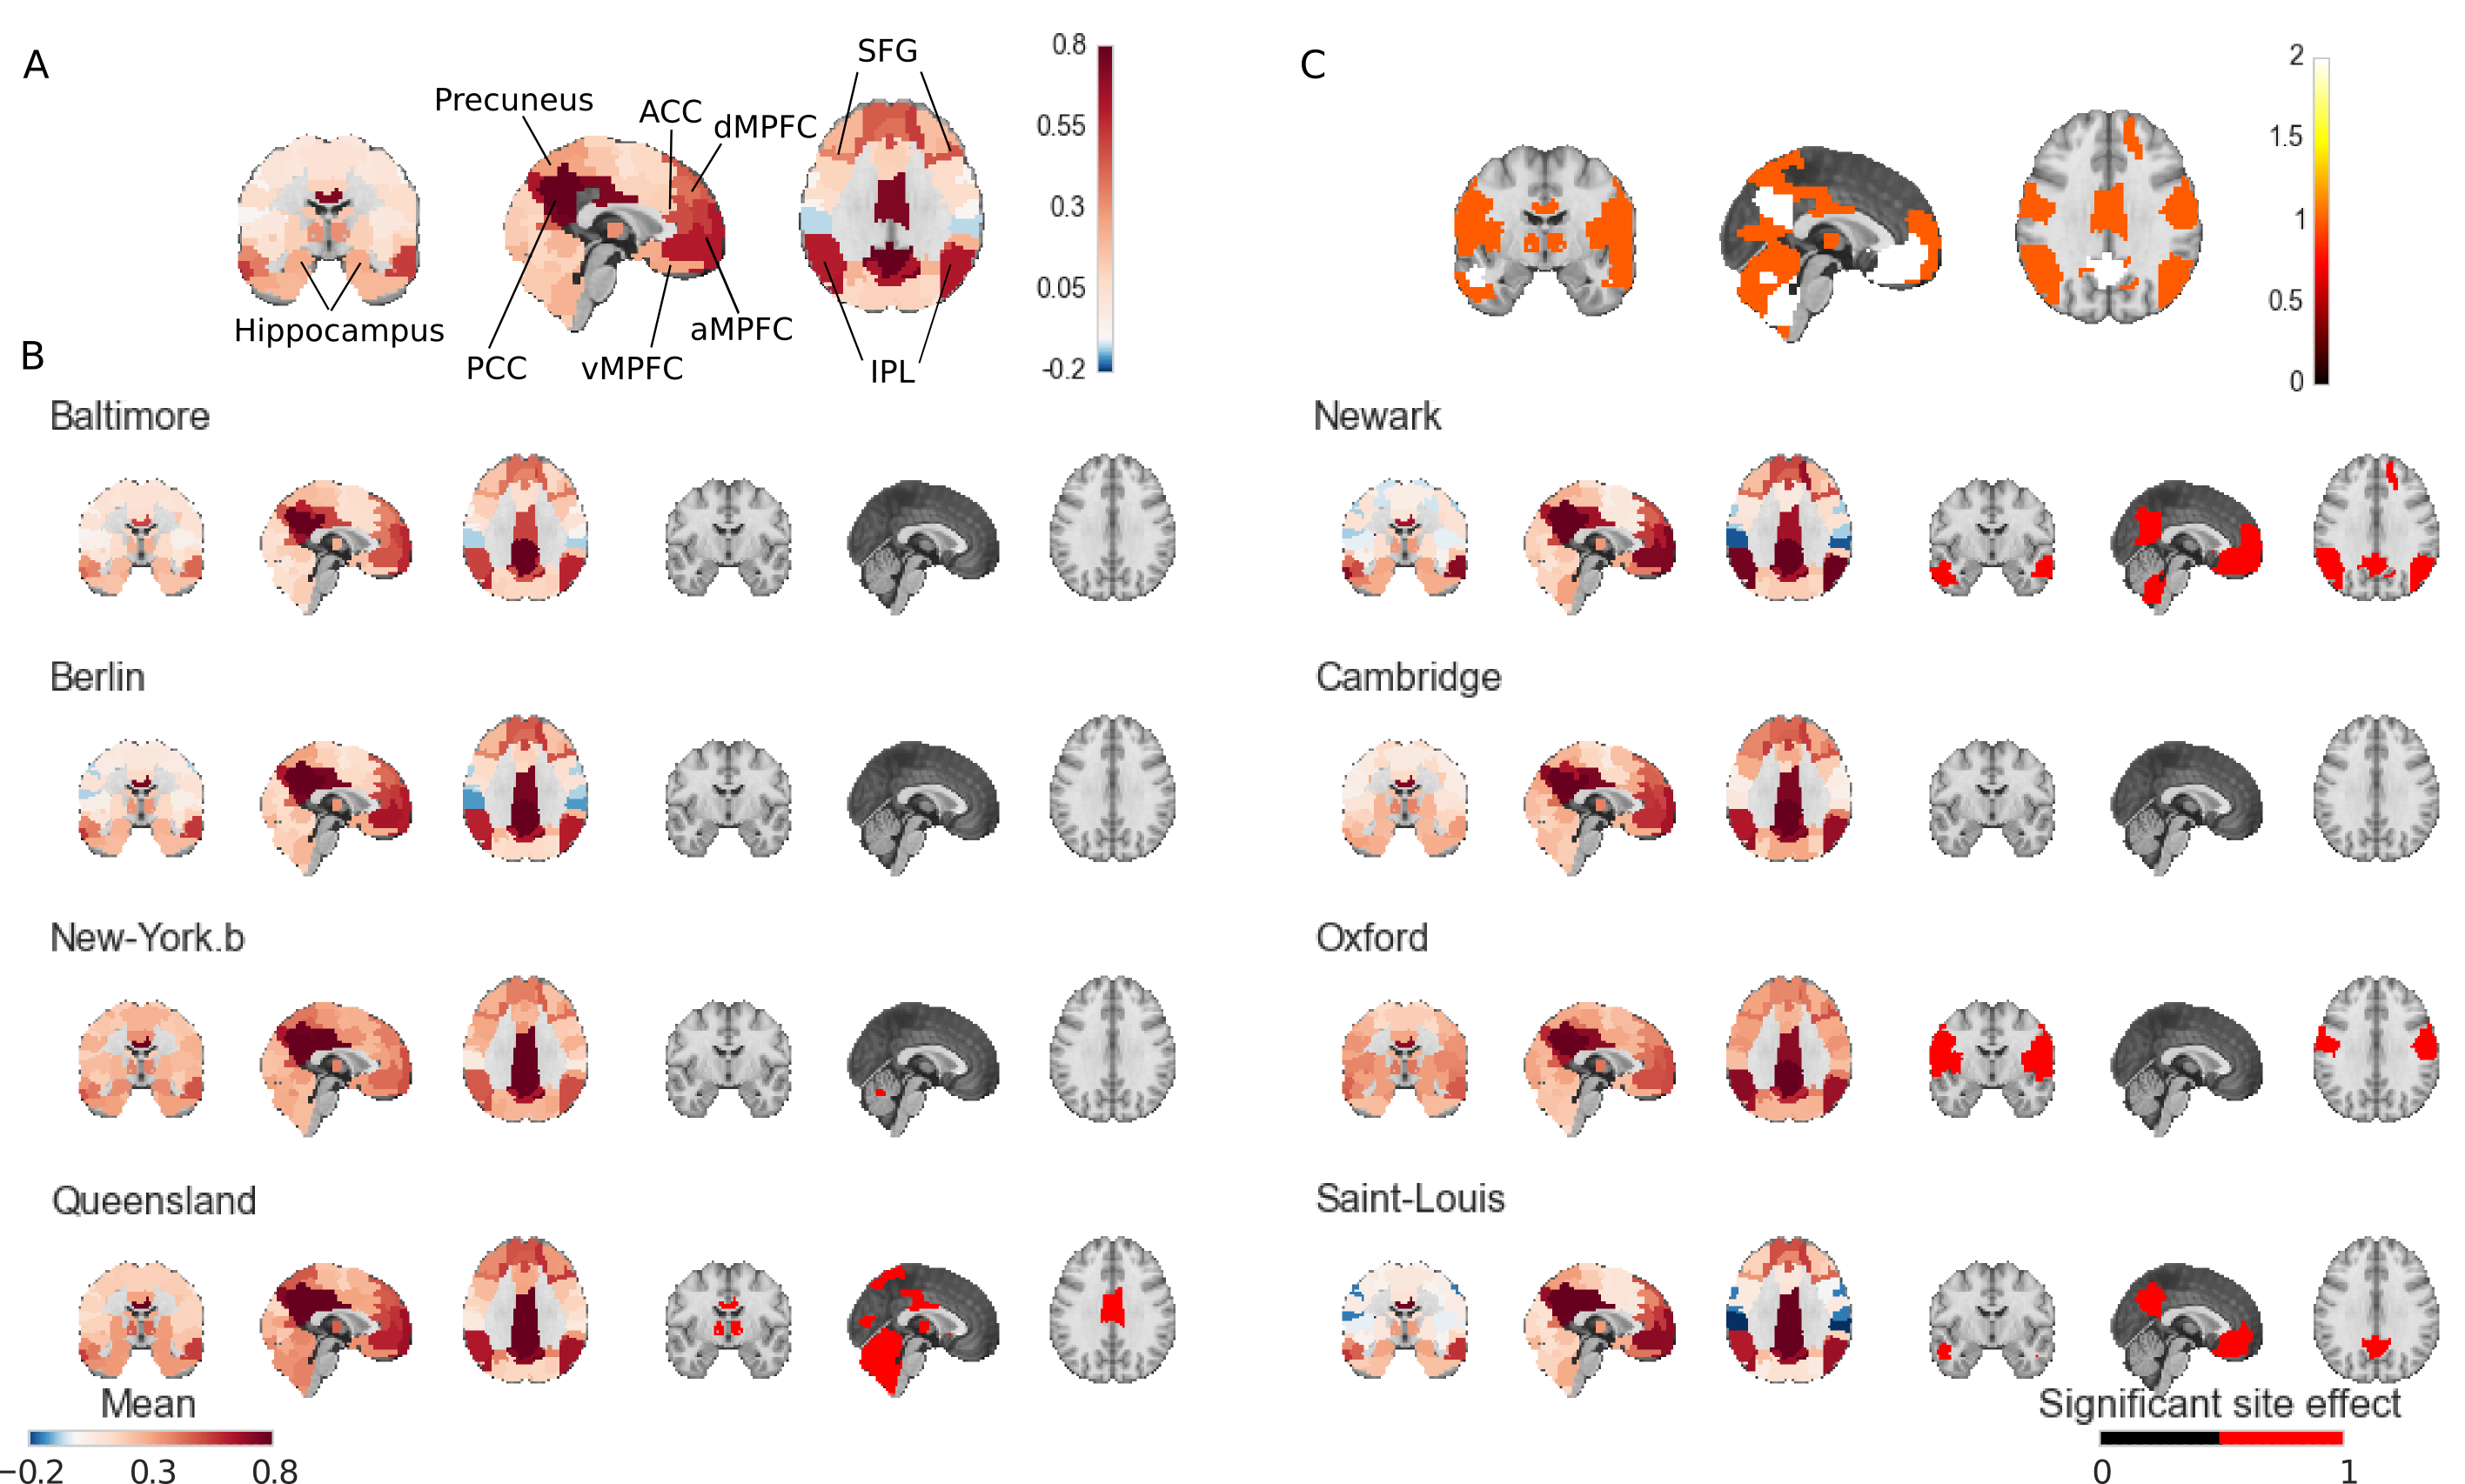
\includegraphics[width=\linewidth]{../figures/dmn_multisite.png}
\end{center}
\caption[DMN variability across sites]{
A) Reference map of the default mode network (DMN) obtained using a seed in the posterior cingulate cortex (PCC). With labels for principal structures of the DMN.
B,C) Average functional connectivity maps of the default-mode network at 8 sites (Baltimore, Newark, Berlin, Cambridge, New-Yorkb, Oxford, Queensland and SaintLouis). The significant differences between the average functional connectivity maps of two sites (called the inter-site bias), along side the statistically significant  differences obtained using a GLM procedure with covariates coding for age, sex and FD for each subject and the p-values were corrected using an FDR procedure ($\alpha=0.05$).
D) A summary for each region of the number of sites showing a significant inter-site difference in the DMN.
}
\label{fig_DMN_variability}
\end{figure}

\paragraph{Site bias in the default-mode network} We first focused on the connections associated with a seed region located in the precuneus (PCC), a key node of the DMN and one of the most widely studied resting-state network \citep{Greicius2004}. The connections were based on the Cambridge 100 parcellation, and were represented as a connectivity map, Figure \ref{fig_DMN_variability}. Panel Figure \ref{fig_DMN_variability}A shows the posterior cingulate cortex (PCC) connectivity map, averaged across all subjects and all sites. The key regions of the DMN are easily identifiable, and include the PCC, precuneus, inferior parietal lobule, anterior cingulate cortex, medial pre-frontal cortex (dorsal, anterior and ventral), superior frontal gyri and the medial temporal lobe \citep{Damoiseaux2006,Dansereau2014,Yan2013a}. The average connectivity map of the DMN was then extracted for each site, Figure \ref{fig_DMN_variability}B,C. Qualitatively, the site-specific DMN maps were very consistent, as expected based on the literature. We then tested for the significance of the site bias, i.e. the difference in average connectivity at a given site and the average connectivity at all remaining sites (FDR corrected for multiple comparisons across the brain, $q<0.05$). A significant bias for at least one region could be identified for every site, without exception, Figure \ref{fig_DMN_variability}B,C. Figure \ref{fig_DMN_variability}D shows how reproducible were the significant bias in connectivity across the brain and sites. The identified location were quite variable, most of them identified at less than three sites.

\begin{figure}[tbp]
\begin{center}
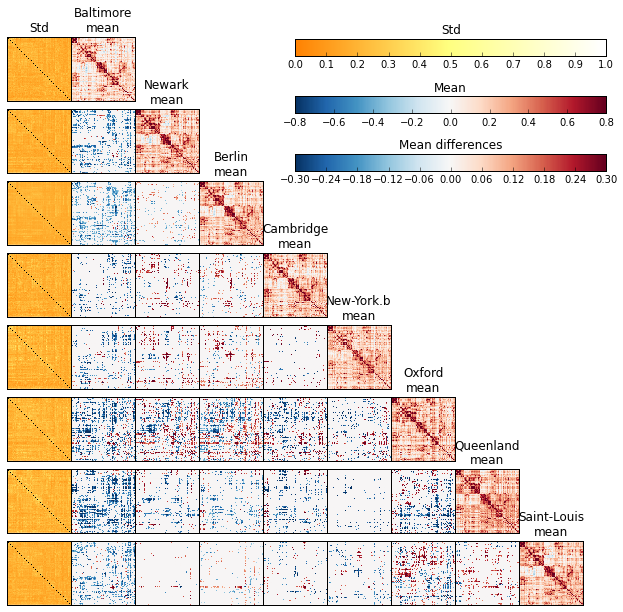
\includegraphics[width=\linewidth]{../figures/connectome_multisite.png}
\end{center}
\caption[Connectome variability across sites]{
A) Average functional connectome of 8 sites (Baltimore, Newark, Berlin, Cambridge, New-Yorkb, Oxford, Queensland and SaintLouis), On the left and top of the matrix a partition in 7 network is color-coded, and the corresponding networks are mapped in B.
B)Partition in 7 networks obtained from a hierarchical clustering (Ward criterion) of the connectome in A. The name of each network is also identified.
C) Average individual site connectomes are shown in C along side the area significantly different from the rest of the sites.
D)Sum of the significant changes in C. Statistical differences are obtained using a GLM procedure include age, sex and FD for each subject with an FDR correction procedure ($\alpha=0.05$).
}
\label{fig_connectome_variability}
\end{figure}


\paragraph{Site bias across the connectome} In order to extend these observations outside of the DMN, we derived the entire connectome using the Cambridge 100 parcellations. Figure \ref{fig_connectome_variability}A shows the average connectome, pooling all subjects and sites together. The regions have been re-ordered based on a hierarchical clustering (with Ward criterion). A network structure is clearly visible as squares of high connectivity on the diagonal of the connectome (as outlined by black lines). Each diagonal square corresponds to the intra-network connectivity for a partition into 7 networks presented in Figure \ref{fig_connectome_variability}D. These 7 networks were consistent with the major distributed resting-state networks reported using cluster analysis in previous work \citep[e.g.,]{Heuvel2008, Bellec2010, Yeo2011, Power2011}. Specifically, the DMN, visual, sensorimotor, dorsal and ventral attentional networks (dATT and vATT, respectively). A mesolimbic network and cerebellar/visual network were also identified. Panel C shows how this large-scale connectome organization varied from site to site. The average connectivity per site as well as significant differences with the average of the remaining sites (FDR corrected at 0.05) is presented in panel C. Visually, consistent with what was observed in the DMN, the organization of the average connectome into large-scale resting-state networks was preserved in all sites. Some significant site effects were still detected in the connectivity both within each network, as well as in the off-diagonal rectangles highlighting between-network connectivity. By counting the frequency of significance of site effects across all 8 sites, it was apparent that significant site effects were quite variable in their localization and spread across the full connectome. 
% The connectome standard deviation across subjects for each site is shown in supplementary material (see \ref{fig_std_connectomes}).

\begin{figure}[tbp]
\begin{center}
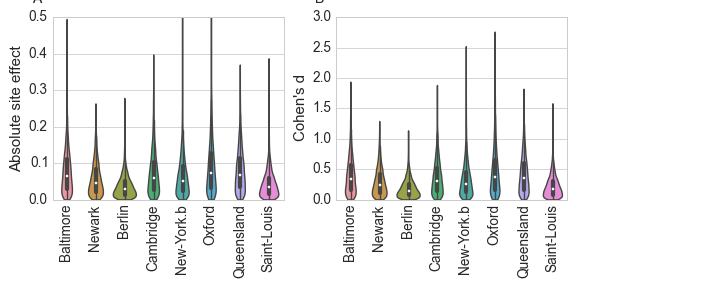
\includegraphics[width=\linewidth]{../figures/boxplot_intra_inter_var.png}
\end{center}
\caption[inter vs. intra site variability]{
Distribution of intra-site (between-subject) standard deviation vs. inter-site (between-site) standard deviation, from a subset of 8 sites from the 1000 functional connectome dataset. A) Detailed intra-site standard deviation for each site. B) Detailed inter-site absolute bias for each site. C) The average intra-site vs. inter-site bias distribution. 
}
\label{fig_site_variability}
\end{figure}

\paragraph{Site bias vs within-site variations across subjects} In order to assess how severe was the amplitude of inter-site bias in resting-state connectivity measures, we compared these measures with the variations across subject within site. This is a standard approach: the Cohen's $d$ measure of effect size \citep{Cohen1992} precisely measures the ratio between the difference in mean between two populations (sites) and the standard deviation of the measure, assumed to be identical in the two populations (sites). Figure \ref{fig_site_variability}A presents violin plots of the distribution of the standard deviation across subjects and all pairs of connections in the Cambridge parcellation, for each site. This distribution was very consistent across sites with a median value near 0.2 and 5\% and 95\% percentiles around 0.1 to 0.3 respectively. Note that the region-to-region maps of within-site across-subjects std are presented for the DMN in Supplementary Figure \ref{fig_std_DMNs}, and for the entire connectome in the Supplementary Material \ref{fig_std_connectomes}. Figure \ref{fig_site_variability}B presents a violin plot of the inter-site bias across all subjects and connections, defined as the absolute difference in mean connectivity between a particular site and the average connectivity across all remaining sites. Again, the distributions were mostly consistent across sites, with a median around 0.5, 5\% percentile near 0 and 95\% percentiles in the 0.2-0.3 range. The median bias across sites was about 0.07, about 3-fold smaller of the median within-site std across participants, which was about 0.2. This effect size would be deemed small-to-moderate, which suggests that the impact of additive inter-site bias on statistical tests will be limited. We then proceeded to formally test this hypothesis using Monte-Carlo simulations. 

\subsection{Simulation of multisite fMRI connectivity}

\begin{figure}[tbp]
\centering
\captionsetup[subfloat]{labelformat=empty}
{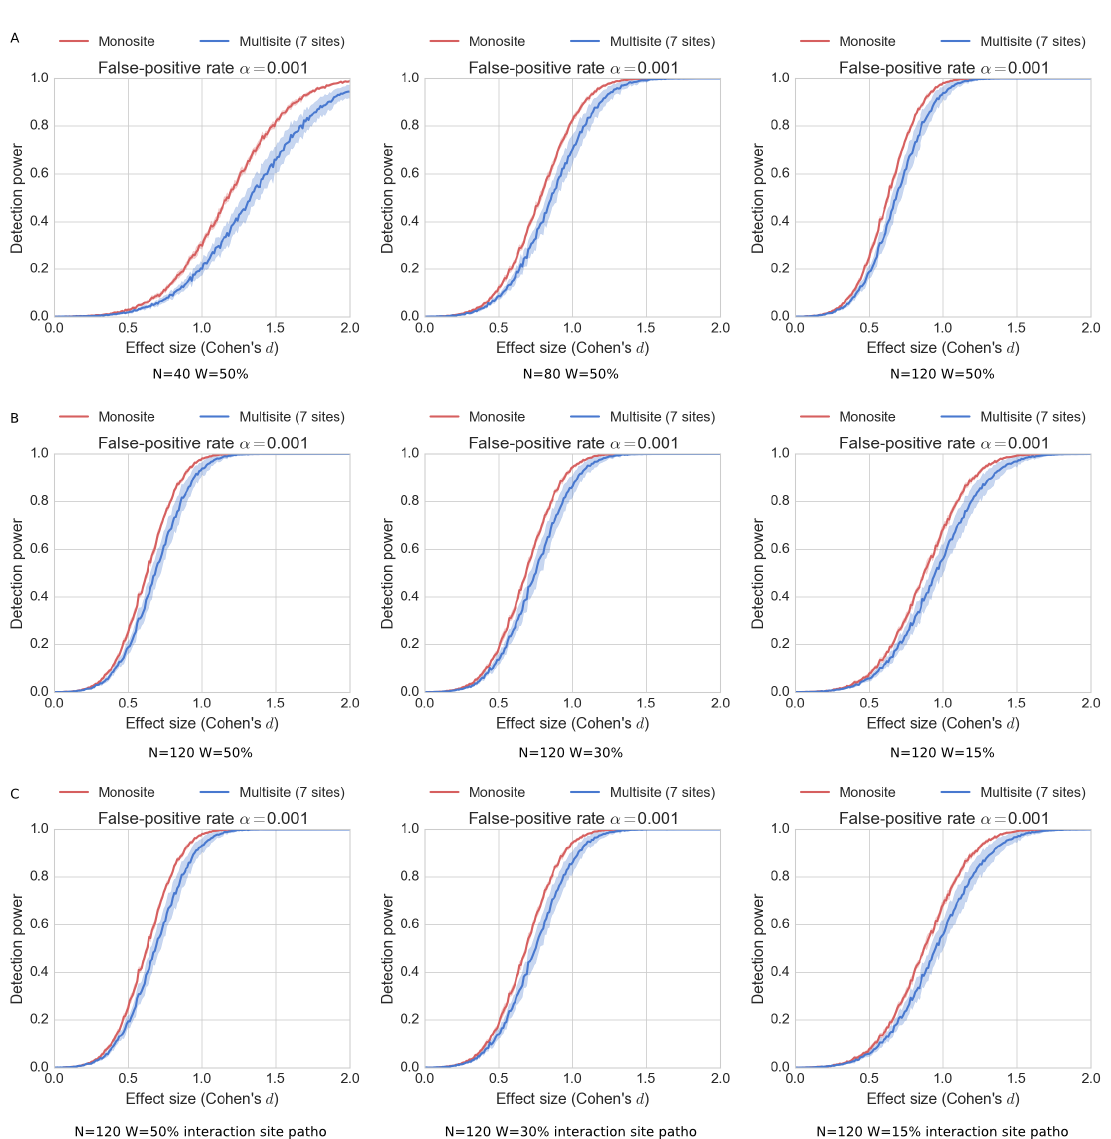
\includegraphics[width=\textwidth]{../figures/simulations_real_7sites.png}}

\caption{
A)Simulation on real data, detection power of two groups with an allocation ratio $W$ of 50\% between the 7 sites. Every plot show two scenarios: 1) monosite and 2) multisite 7 sites with correction for multisite differences using dummy variables. Each plot show the detection power in function of the effect-size for 3 different sample size 40, 80 and 120 subjects in total.
B)Simulation on real data, detection power of two groups for a total of 120 subjects between 7 sites. Every plot show two scenarios, 1) monosite and 2) multisite 7 sites with correction for multisite differences using dummy variables. Each plot show the detection power in function of the effect-size for 3 different allocation ratio $W$ of 50\%, 30\% and 15\% for each simulation.
}
\label{fig_real_sim}
\end{figure}

\paragraph{Statistical power and effect size} Figure \ref{fig_real_sim}A shows the relationship between effect size and sensitivity, for different sample size and in a single site vs multisite (7 sites) settings. In the multisite simulations, all sites had the same sample size, and half of the subjects were assigned to the ``patients'' group ($w=0.5$). The average and std of sensitivity was plotted across the 11 selected connections. As expected, the sensitivity increased with sample size, quite markedly. in multisite simulations , for an effect size of 1, generally considered as a large effect, the detection of significant group differences (false-positive rate $\alpha=0.001$) had a 20\% sensitivity with 40 subjects , 80\% sensitivity with 80 subjects and almost 95\% sensitivity with 120\% subjects. The sensitivity was larger in single site than multisite simulations, yet the difference between the two decreased when the sample size increased. With 40 subject and an effect size of 1, the single site detection had close to 30\% sensitivity, compared to 20\% for the multisite simulations. With 120 subjects, still for an effect size of 1, the difference in sensitivity was only a few percent. The same trend was apparent for all tested effect sizes. 

\paragraph{Statistical power and group allocation ratio} Figure \ref{fig_real_sim}B shows the effect of debalancing the two groups at various allocation ratio $W$ (50\% , 30\% and 15\%), all simulations being performed with a sample size $N=120$  subjects. Has we increase the debalancing our ability to detect a particular effect-size is diminished. As an example for an effect-size of 1 we would detect the effect in 95\% of the cases in a 50\%-50\% balanced scenario, this would go down to 90\% in a 30\%-70\% scenario and to 65\% in a 15\%-85\% scenario. Although the debalancing effect  is observed in both monosite and multisite scenarios. An optimal allocation ratio would therefore be a 50\%50\% for multisite and monosite study.



\begin{figure}[tbp]
\centering
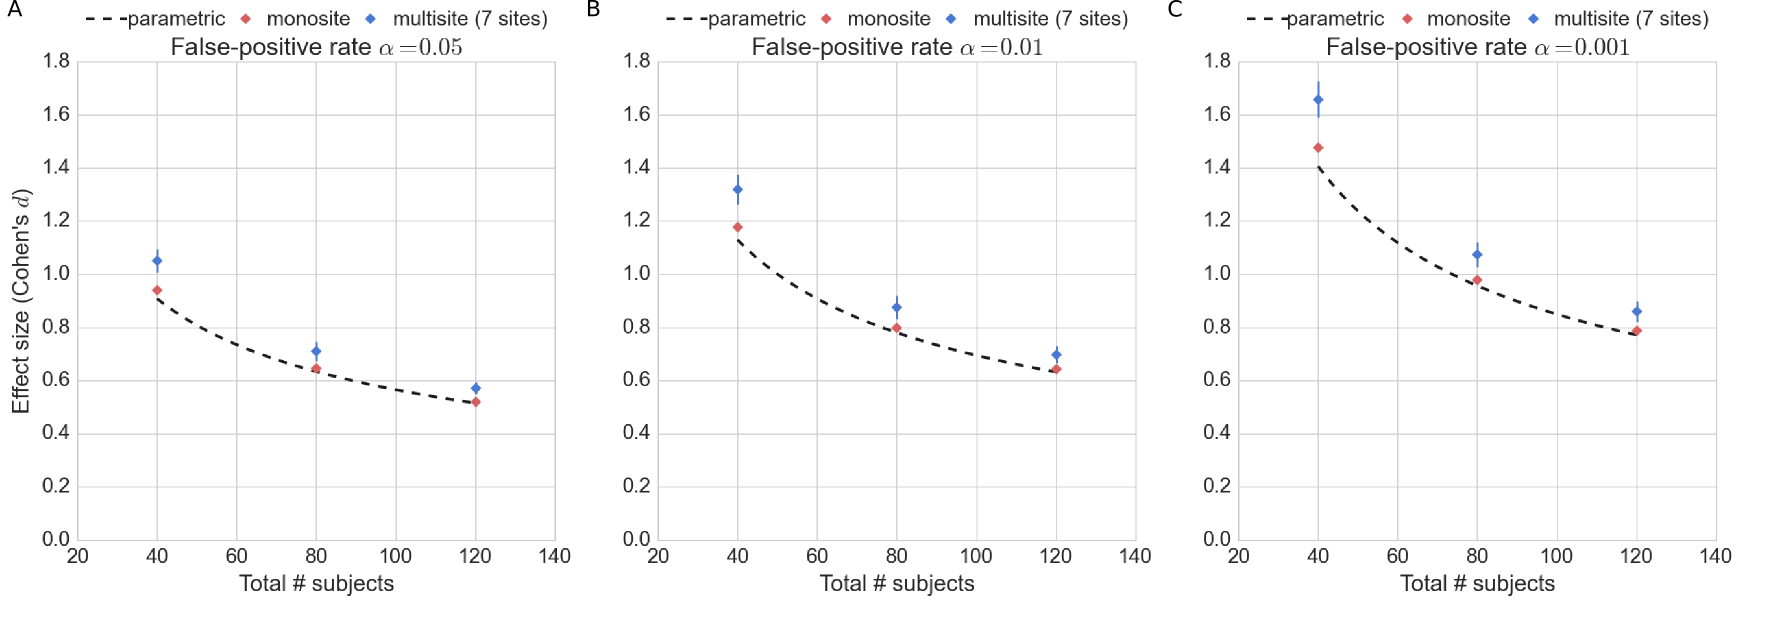
\includegraphics[width=\textwidth]{../figures/samplesize_x_effectsize.png}
\caption[]{
Sample-size in function of the effect-size for a detection power of 80\%
A) using a threshold on the probability of having false-positive rate ($\alpha=0.05$) on a balanced dataset using an allocation ratio $W$ of 50\%.
B) using a threshold on the probability of having false-positive rate ($\alpha=0.01$) on a balanced dataset using an allocation ratio $W$ of 50\%.
C) using a threshold on the probability of having false-positive rate ($\alpha=0.001$) on a balanced dataset using an allocation ratio $W$ of 50\%.
The monosite performance in red and the multisite in blue. In black the dotted line show the parametric estimation of the effect size for the given sample-size.
}
\label{fig_sampeffect_curves_alpha001}
\end{figure}

\paragraph{Detectable effect size, as a function of sample size} To summarize the previous findings plot of the sample-size in function of the effect-size for a detection power of 80\% is shown in Figure \ref{fig_sampeffect_curves_alpha001}.As we can see the parametric estimation follow nicely the monosite estimation although a bit underestimated on small sample-size. This is also the case for multisite estimation where a delta of 0.25 Cohen's $d$ was found at 40 subjects. This delta diminish inversely proportional to the sample-size to reach a delta of around 0.1 at 120 subjects. The Cohen's $d$ achieve for a given sample-size is also more variable among connections with 40 subjects (std=0.05) compared to 120 subjects (std=0.025). As previously noted the lowest detectable effect size for a sensitivity of 80\% is about 0.8, at a single site with 120 subjects. At this sample size, the difference between single and multisite studies appear to be marginal only, with only a few percent of difference in detectable effect sizes. 



%%%%%%%%%%%%%%%%%%%%%%%%%%%%%%%%%%%%%%%%%%%%%
% END of results section                    %
%%%%%%%%%%%%%%%%%%%%%%%%%%%%%%%%%%%%%%%%%%%%%

\section{Conclusions and discussion}

\paragraph{Inter-site bias in rs-fMRI connectivity} Typical resting-state networks were reliably found across sites, such as the DMN, the vATT, dATT, Visual and SM networks. This was strongly expected given the relative consistency of their distribution across individuals, studies, preprocessing approaches or even methods used to extract networks \citep{Damoiseaux2006,vandeheuvel2008,Bellec2010c,Yeo2011,Power2011}. We however found that significant differences in average connectivity (bias) existed between the sites, as previously reported by \citep{Yan2013a}. This connectivity bias may undermine the generalization of the results derived at a single site. The inter-subject (intra-site) standard deviation of the connections was found to be 2 fold greater than the inter-site absolute bias. This effect size measured in Cohen's d would be deemed small-to-moderate, which suggests that the impact of additive inter-site bias on statistical tests will be limited. A reassuring finding in favor of the feasibility of statistical tests pooling fMRI data across multiple sites.\\


\paragraph{Spatial distribution of connectivity bias} We found that the brain connections exhibiting significant inter-site bias were quite variable, with most of them identified in less than one fourth of the sites. This suggests that there are no large network-specific inter-site bias or that the statistical power for detecting bias with the employed site sample size was limited. Looking at the spatial location of the site bias with respect to a partition in 7 networks, we noticed that the DMN and the dATT networks were less affected by site bias then the cerebellar, mesolimbic and sensory-motor networks \emph{did we really observe that? CD: Yes looking at the matrix of figure2D I could observe a bit more difference from one network to the other I can compute the average of the value in each network that would give use a cleaner picture... }. This last finding may be associated with the fact that those network are more on the periphery of the brain and may be more sensitive to motion artifacts. 

\paragraph{Statistical power and multisite rs-fMRI} The multisite simulation polling 7 sites showed, after accounting for site-related differences (explicit correction for multi-site variability using dummy variables), similar detection power although slightly lower for the multisite configuration. However, the difference between a monosite and a multisite study was smaller as we increase the sample size. Another compelling proof of the lack of statistical power at small sample sizes is the study reported by \cite{Nielsen2013} where they did an analysis on a single site dataset and a multi-site dataset of subject with autism and concluded that the multi-site autism study classification accuracy significantly outperformed chance but was much lower for multi-site prediction than for previous single site results. We therefore need to keep in mind that the site effect must be taken in account in the analysis and that we may suffer a small lost in detection power for a given effect-size in a multisite configuration compared to an equal size monosite study.\\
\par
Second for a given detection power the lowest effect-size that we are able to detect is more variable across connections for a low sample-size and decrease as we increase the sample-size.  
An observation promoting the use of large sample-size ($>100$ subjects) for multisite studies. Note that this is probably greatly influence by the number of sites that one will pool to achieve a final given sample-size. 

%Second the Cohens's $d$ achieve for a given sample-size is also a lot more variable among connections with low sample-size compared to larger sample-size \emph{This sentence is crytpic. Beyond the form, what may cause that?}. \emph{Resulting in the following conclusion combining large site may results in low bias compared to very small sites. It is therefore better to have a few large sites then a large number of small sites.I am pretty sure we did not test that. We had 7 small vs 7 large sites. We did not compare a few sites vs many sites with the same sample size}. 

%\par
%\emph{At this stage, you are done discussing your findings in direct relationship with your objectives. Now is time to discuss limitations, implications and also potential avenues of future work}. 

\paragraph{Statistical power and sample size} For an effect size considered as medium, e.g. 0.5, the sensitivity was low (below 20\%), even for monosite simulations with 120 subjects (Figure \ref{fig_real_sim}A). This is a sobering reminder that with the low false-positive rate typically used in rs-fMRI studies, resulting from correction for multiple comparisons, the sensitivity is quite limited even for over 100 subjects. In particular, our results suggest that resting-state studies based on 40 subjects or less, even at a single site, may be seriously under-powered, unless the effect under investigation were extremely large (Cohen's $d$ greater than 1.5). Also in both cases (monosite and multisite) the effect of unbalancing the two populations may greatly reduce our capacity to detect changes e.g. for an effect size of 1 the detection power goes from 95\% in a balanced case to 65\% for an unbalanced dataset (allocation ratio W=15\%). We therefore recommend to favor balanced dataset when pooling them in order to reduce the variance.

\paragraph{Underlying causes of the site bias}

Not all sites seemed to be equally biased, with sites like Berlin or Saint-Louis showing a small number of connections significantly different then the grand average connectivity matrix, while sites like Baltimore, Queensland and Oxford showed much more biased connectivity measures. This may simply be a statistical fluke or a reflection of the protocol or scanner characteristics of these sites. Multiple cause may be interacting together to produce the site bias, like reported by \cite{Yan2013a}, although some of these sources of variance could be better controlled like the scanner parameters paired with the use of a phantom to promote more homogeneous configurations across site and a close monitoring of the experimental paradigm across-site as proposed by \cite{Friedman2006,Friedman2006a,Glover2012}. Although even in standardized study with a great effort made on homogenizing the scanners protocol differences remain \cite{Brown2011}. A much larger site sample with varying parameters could enable a data-driven identification of the critical parameters impacting site bias. The various releases made by the INDI may fill that gap in the literature in the future, as the scanner protocols are much better described in recent releases such as CoRR than they were in the initial FCP release. There will however still be a bias that may be related to local recruitment strategies, the characteristics of local population, or undocumented aspects of the study such as training of subjects to the scanning environment. Many physiological factors are likely to be contributing to these variations, such as the cognitive state of the subject, the level of alertness/drowsiness, circadian rhythm, hunger, medical regimen, potential neurostimulants, amongst others. 

Our study show simulation using real data of heterogeneous protocols on 7 scanners compared to the majority of the literature on the subject comparing two sites homogeneous sites \citep{Costafreda2007,Suckling2008,Sutton2008,Glover2012} and three sites for \cite{Gountouna2010}. As opposed to \cite{Sutton2008,Brown2011} who reported a 10 times smaller contribution of the inter-site variance, we have observed a 2 times smaller contribution. There is mainly 2 factors that may contribute to an increase in site variance and explain this difference in site variation, namely the number of sites involved in the study and the degree of homogenization of the protocols and experiments. Also a word of caution should be made regarding the fact that the great majority of scanner were Siemens, and therefore more variability may be found using various scanner manufacturer unfortunately this avenue was not testable using this dataset.

\paragraph{Other types of multisite data} An other limitation is in the case of very large number of site with a few subjects per site, which is common for the recruitment of patient populations in a limited time frames, e.g. the Alzheimer’s disease neuroimaging initiative (ADNI) \citep{Mueller2005} and fBIRN \citep{Friedman2006,Friedman2006a}, and in pharmaceutical clinical trials at phase II and III \footnote{\url{http://www.roche-trials.com/trialDetailsGet.action?studyNumber=BP28248}}. An important benefit of multisite acquisitions is to offer improved generalization compared to single site studies, due to more diversity in scanners and populations. In this case the multisite effect may be more pronounce then what we observed with 7 sites, although the detection power between monosite and multisite diminish with the sample size and may be negligible for samples greater then 200 subjects. Unfortunately this hypotheses could no be tested with the current dataset due to the limited number of sites available. In future work given an appropriate dataset it would be interesting, using a similar approach, to test if the added variability introduce by the use of a large number of sites with a small number of subjects/site will be compensated by the sample size as hypothesized in this study.


\paragraph{Beyond additive bias} Also the generative model used for our simulations was based on the hypotheses of an additive effects of the pathology and site, therefore the results and conclusions can only be valid if the model investigated is in fact an additive effect model. Other effects types may include but are not limited to interactions of the site and pathology, polynomial and non-linear interaction.

\section{Acknowledgments}
Parts of this work were presented at the 2013 annual meetings of the organization for human brain mapping, as well as the  Alzheimer's Association International Conference (AAIC) (2013) (Boston) \citep{Dansereau2013b}. The authors are grateful to the members of the 1000 functional connectome consortium for publicly releasing there dataset. The computational resources used to perform the data analysis were provided by ComputeCanada\footnote{\url{https://computecanada.org/}} and CLUMEQ\footnote{\url{http://www.clumeq.mcgill.ca/}}, which is funded in part by NSERC (MRS), FQRNT, and McGill University. This project was funded by NSERC grant number RN000028, a salary award from ``Fonds de recherche du Qu\'ebec -- Sant\'e'' to PB as well as a salary award by the Canadian Institute of Health Research to CD.

\section*{References}

\bibliographystyle{elsarticle-harv}
\bibliography{cdansereau}


\pagebreak



\clearpage
\appendix


%% SUPPLEMENTARY MATERIAL
\clearpage
\pagebreak
\renewcommand{\thefigure}{S\arabic{figure}}
\renewcommand{\thetable}{S\arabic{table}}
\setcounter{figure}{0}
\begin{center}
\emph{Supplementary Material {--} Statistical power and measurement bias in multisite resting-state fMRI connectivity}\\

\vspace{\baselineskip}Submitted to Neuroimage.\\

\vspace{\baselineskip}C. Dansereau$^{1,2}$,  Y. Benhajali$^{1}$,C. Risterucci$^{3}$, E. Merlo Pich$^{3}$, P. Orban$^{1}$, D. Arnold$^{4}$, P. Bellec$^{1,2}$\\

\end{center}
$^1$Functional Neuroimaging Unit, Centre de Recherche de l'Institut Universitaire de G\'eriatrie de Montr\'eal\\
$^2$Department of Computer Science and Operations Research, University of Montreal, Montreal, Quebec, Canada\\
$^3$F. Hoffmann-La Roche Ldt., Basel, Switzerland\\
$^4$NeuroRx, Montreal, Quebec, Canada\\

For all questions regarding the paper, please address correspondence to Pierre Bellec, CRIUGM, 4545 Queen Mary, Montreal, QC, H3W 1W5, Canada. Email: pierre.bellec (at) criugm.qc.ca.\\

\section*{Supplementary Material} 

\begin{figure}[tbp]
\centering
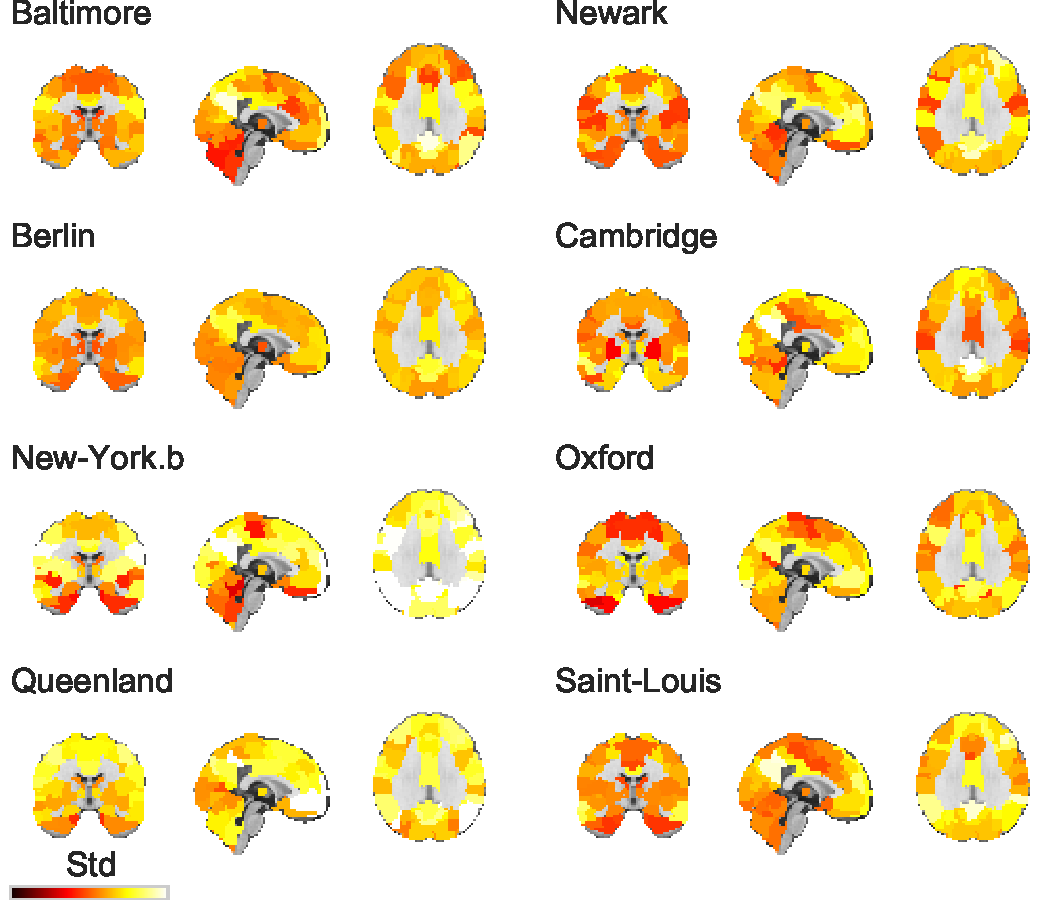
\includegraphics[width=0.75\textwidth]{../figures/dmn_stdmultisite.pdf}
\caption[]{
Overlay of the standard deviation of the DMN for each site on the MNI152 template.
}
\label{fig_std_DMNs}
\end{figure}

\begin{figure}[tbp]
\centering
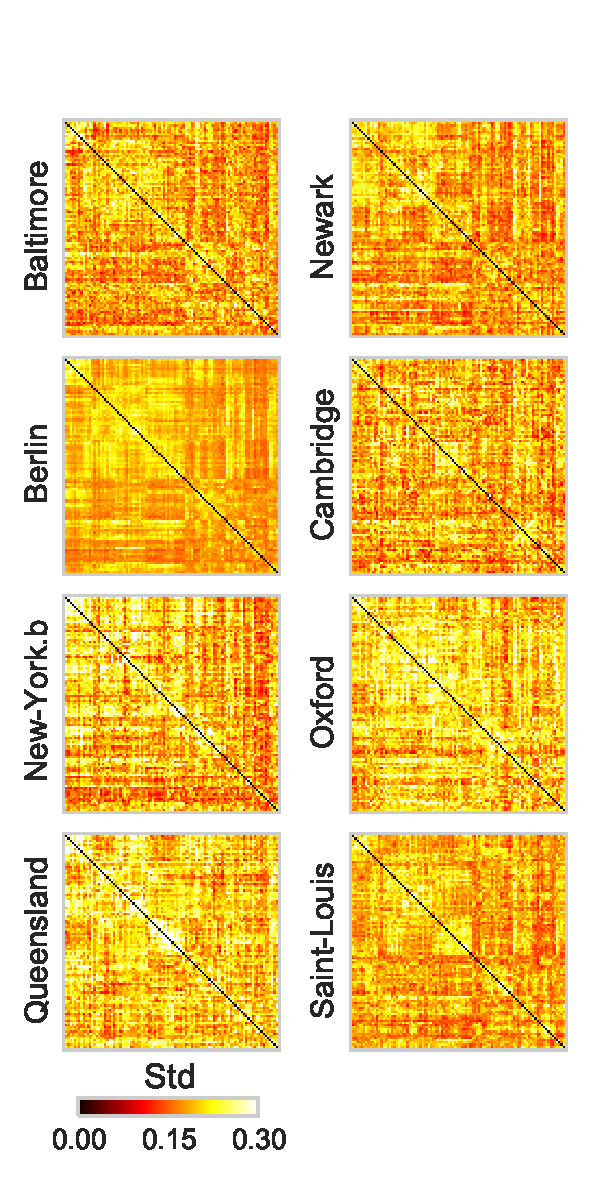
\includegraphics[width=0.50\textwidth]{../figures/connectome_std_multisite2.pdf}
\caption[]{
The standard deviation of the connectome for each site.
}
\label{fig_std_connectomes}
\end{figure}


Figure \ref{fig_real_sim_debalancing_2sites} show a scenario of two sites one large (80 subjects) and one small ($\sim20$ subjects) unbalanced at an allocation ratio $W$ of 30\% and the inverse ($W=$70\%). As we can see the multisite configuration is as good as the monosite and the variance between connection is of the same order for the monosite and multisite.

\begin{figure}[tbp]
\centering
\captionsetup[subfloat]{labelformat=empty}
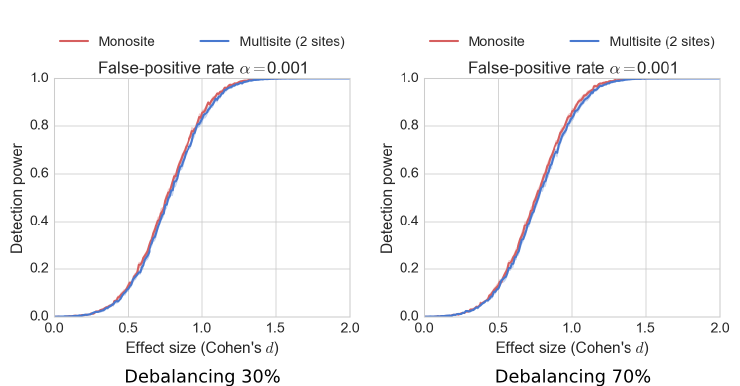
\includegraphics[width=.75\textwidth]{../figures/simulations_real_2sites.png}
\caption{
Simulation on real data, detection power of two groups for a total of 100 subjects between 2 sites, one small site of 20 subjects and one large of 80 subjects. Every plot show two scenarios, 1) monosite and 2) multisite 2 sites with correction for multisite differences using dummy variables. Each plot show the detection power in function of the effect-size for 2 different allocation ratio $W$ of 30\% and 70\% between 2 sites.
}
\label{fig_real_sim_debalancing_2sites}
\end{figure}


\end{document}


